\documentclass[conference]{IEEEtran}
\IEEEoverridecommandlockouts

\usepackage{cite}
\usepackage{amsmath,amssymb,amsfonts}
\usepackage{algorithmic}
\usepackage{graphicx}
\usepackage{textcomp}
\usepackage{xcolor}
\usepackage{booktabs}
\usepackage{multirow}
\usepackage{hyperref}
\usepackage{url}
\usepackage{subcaption}

\def\BibTeX{{\rm B\kern-.05em{\sc i\kern-.025em b}\kern-.08em
    T\kern-.1667em\lower.7ex\hbox{E}\kern-.125emX}}

\begin{document}

\title{Reproducibility and Improvement Study of LITETime for Time Series Classification}

\author{
\IEEEauthorblockN{Kiran Meenakshi Sundaram}
\IEEEauthorblockA{\textit{School of Computer Science} \\
\textit{University College Dublin}\\
Ireland \\
kiran.meenakshisundaram@ucdconnect.ie}
\and
\IEEEauthorblockN{Jos\'e Ram\'on Morera Campos}
\IEEEauthorblockA{\textit{School of Computer Science} \\
\textit{University College Dublin}\\
Ireland \\
jose.moreracampos@ucdconnect.ie}
\and
\IEEEauthorblockN{Pelayo Garc\'ia \'Alvarez}
\IEEEauthorblockA{\textit{School of Computer Science} \\
\textit{University College Dublin}\\
Ireland \\
pelayo.garciaalvarez@ucdconnect.ie}
}

\maketitle

\begin{abstract}
Time Series Classification (TSC) is a fundamental task in machine learning with applications spanning healthcare monitoring, industrial automation, and activity recognition. While deep learning models have achieved strong benchmark performance, many require substantial computational resources, limiting deployment in resource-constrained environments. Lightweight architectures such as LITE and its ensemble variant LITETime address this gap by combining trainable and non-trainable convolutional filters to reduce parameter complexity. In this study, we reproduce the published LITETime results on the full 128-dataset UCR archive, achieving a mean accuracy of 0.8316 compared to the reported 0.8304, confirming reproducibility. We then evaluate targeted improvements on a representative 31-dataset fast subset, finding that global z-normalization yields the largest gain (0.9038 vs.\ 0.8950 baseline, +0.88\%), followed by the AdamW optimizer (+0.23\%). We further extend the evaluation to multivariate time series classification, comparing LITE and LITEMV against state-of-the-art methods on 30 datasets. An analysis of ensemble size reveals diminishing returns beyond five members. Our results confirm the reliability of LITETime and demonstrate that meaningful performance improvements can be achieved through optimization strategies without modifying the core architecture. All code and results are publicly available.\footnote{\url{https://github.com/jose-r-morera/LITE}}
\end{abstract}

\begin{IEEEkeywords}
time series classification, deep learning, reproducibility, lightweight neural networks, ensemble methods
\end{IEEEkeywords}

%=============================================================================
\section{Introduction}
%=============================================================================

Time series classification (TSC) is a core task in modern data-driven systems. Sequential observations recorded over time---electrocardiogram (ECG) signals, wearable sensor data, motion capture recordings, and industrial equipment telemetry---exhibit temporal dependencies that must be captured effectively for accurate classification.

Early TSC approaches relied on distance-based methods such as Dynamic Time Warping (DTW) combined with nearest-neighbor classification~\cite{keogh2001dtw}. While effective, these methods required handcrafted features and scaled poorly to large datasets. The emergence of deep learning introduced architectures capable of learning hierarchical temporal features directly from raw data~\cite{fawaz2019deep}.

Deep convolutional architectures---Fully Convolutional Networks (FCN)~\cite{wang2017fcn}, Residual Networks (ResNet)~\cite{wang2017fcn}, and InceptionTime~\cite{fawaz2020inceptiontime}---have achieved state-of-the-art performance on many benchmarks. However, their high computational cost and large parameter counts make them impractical for real-time or embedded applications.

To address these limitations, Ismail-Fawaz et al.\ proposed LITE (Light Inception with boosTing tEchniques), a lightweight architecture that combines trainable and non-trainable convolutional filters with depthwise separable convolutions to significantly reduce the parameter count~\cite{ismail2024lite}. LITETime extends this by ensembling multiple LITE models, improving robustness against random initialization effects.

In this project, we pursue three objectives: (1)~reproduce the published LITETime results on the full UCR archive to validate the original findings, (2)~evaluate targeted improvements including optimizer selection, normalization strategies, and batch-size tuning, and (3)~extend the evaluation to multivariate time series classification. The main contributions are:

\begin{itemize}
    \item Independent reproduction of LITETime on all 128 UCR datasets, confirming the published accuracy within 0.15\%.
    \item Construction of a stratified 31-dataset fast subset for efficient experimentation.
    \item Evaluation of global z-normalization, AdamW optimizer, and batch-size effects, with z-normalization achieving the largest improvement (+0.88\%).
    \item Extension to multivariate TSC on 30 datasets, comparing LITE, LITEMV, and state-of-the-art methods.
    \item Analysis of ensemble size effects, showing diminishing returns beyond 5 members.
    \item Open-source repository with reproducible experimental pipeline.
\end{itemize}

%=============================================================================
\section{Motivation and Impact}
%=============================================================================

The selection of LITETime for this study was motivated by its strong relevance to efficient deep learning for TSC. In real-world deployments---wearable health monitors, industrial fault detectors, edge-based sensor networks---computational resources are limited. Lightweight models enable real-time inference while maintaining competitive accuracy, making them essential for practical machine learning deployment.

The growing importance of reproducibility in AI research further motivated this work. Many published studies report strong results, but independent reproduction can be challenging due to differences in preprocessing pipelines, random seeds, hardware, and software environments~\cite{pineau2021reproducibility}. Reproducibility ensures that scientific findings are reliable and transferable.

This project contributes to the ML community by: (1)~validating the performance claims of a lightweight architecture, (2)~identifying practical optimization strategies that improve performance without architectural modifications, and (3)~providing an open-source benchmark pipeline that can be reused for future studies.

%=============================================================================
\section{Related Work}
%=============================================================================

\textbf{Classical methods.} Distance-based approaches such as DTW with nearest-neighbor classification remain competitive baselines~\cite{bagnall2017bakeoff}. Shapelet-based methods~\cite{lines2012shapelet} extract discriminative sub-sequences, while dictionary methods such as BOSS leverage symbolic representations.

\textbf{Kernel methods.} ROCKET~\cite{dempster2020rocket} introduced random convolutional kernels combined with linear classifiers, achieving state-of-the-art accuracy with exceptionally low training times. MiniRocket~\cite{dempster2021minirocket} and MultiRocket~\cite{tan2022multirocket} further refined this approach.

\textbf{Deep learning.} FCN and ResNet~\cite{wang2017fcn} demonstrated that convolutional architectures can learn useful temporal representations without manual feature engineering. InceptionTime~\cite{fawaz2020inceptiontime} introduced multi-scale convolutional modules with ensemble averaging, achieving leading benchmark performance but at high computational cost.

\textbf{Lightweight architectures.} LITE~\cite{ismail2024lite} addresses the computational limitations of InceptionTime by combining hand-crafted non-trainable filters (for predefined temporal operations) with trainable filters, plus depthwise separable convolutions to reduce parameter counts. LITETime ensembles multiple LITE models to improve robustness.

\textbf{Multivariate TSC.} For multivariate time series, models such as ConvTran~\cite{foumani2023convtran} and Disjoint-CNN~\cite{zhao2017cnn_tsc} have been proposed alongside LITEMV, the multivariate variant of LITE.

%=============================================================================
\section{Architecture Overview}
%=============================================================================

The LITE architecture consists of three main components, as illustrated in Fig.~\ref{fig:architecture}.

\textbf{Hybrid inception module.} The first layer combines three parallel branches of trainable 1D convolutions (with kernel sizes $k$, $k/2$, $k/4$ where $k=40$) with a non-trainable hybrid filter bank. The hybrid filters perform three types of fixed temporal operations: increasing detection (alternating $+1/-1$ patterns), decreasing detection (alternating $-1/+1$ patterns), and peak detection (Mexican hat-like wavelets). These 17 non-trainable filters capture fundamental signal patterns without requiring gradient updates, reducing the trainable parameter count while providing rich temporal features. The outputs are concatenated, batch-normalized, and activated with ReLU.

\textbf{Depthwise separable convolution blocks.} Two subsequent layers use depthwise separable convolutions with increasing dilation rates ($d=2, 4$). Separable convolutions factorize standard convolutions into depthwise and pointwise operations, further reducing parameters. Dilation expands the receptive field without increasing kernel size, enabling the model to capture longer-range dependencies.

\textbf{Classification head.} Global average pooling reduces the temporal dimension, and a dense softmax layer produces class probabilities.

\textbf{LITETime ensemble.} LITETime averages the softmax predictions of $N$ independently trained LITE models (default $N=5$). This reduces sensitivity to random weight initialization and improves classification robustness.

\begin{figure}[htbp]
    \centerline{
\includegraphics[width=\columnwidth]{../../images/LITE.png}}
    \caption{The LITE architecture. Trainable convolutions (blue) are combined with non-trainable hybrid filters (green) in the inception module, followed by depthwise separable convolution blocks with dilation. Source:~\cite{ismail2024lite}.}
    \label{fig:architecture}
\end{figure}

%=============================================================================
\section{Methodology}
%=============================================================================

\subsection{Reproduction Setup}

To reproduce the original results, we used the authors' open-source implementation\footnote{\url{https://github.com/MSD-IRIMAS/LITE}} with the training configuration shown in Table~\ref{tab:config}. Datasets were loaded using the \texttt{aeon} toolkit~\cite{aeon2024}, which provides standardized access to the UCR archive~\cite{dau2019ucr}. Each single LITE model was trained for 1500 epochs with early stopping via checkpoint selection on training loss. LITETime accuracy was computed by ensembling the softmax outputs of 5 independent runs. All experiments were conducted on an NVIDIA RTX 4070 GPU.

\begin{table}[htbp]
\caption{Training Configuration Parameters}
\label{tab:config}
\centering
\begin{tabular}{ll}
\toprule
\textbf{Parameter} & \textbf{Value} \\
\midrule
Optimizer & Adam (baseline) \\
Learning rate & $10^{-3}$ (with ReduceLROnPlateau) \\
LR reduction factor & 0.5, patience 50 \\
Minimum LR & $10^{-4}$ \\
Batch size & 64 \\
Epochs & 1500 \\
Loss function & Categorical cross-entropy \\
Normalization & Per-sample z-normalization \\
Ensemble size ($N$) & 5 \\
\bottomrule
\end{tabular}
\end{table}

\subsection{Fast Subset Construction}

Running all 128 UCR datasets is computationally expensive. To enable efficient improvement experiments, we constructed a representative fast subset of 31 datasets, stratified by training set size, time series length, and number of classes:

\begin{table}[htbp]
\caption{Fast Subset Stratification}
\label{tab:subset}
\centering
\small
\begin{tabular}{lll}
\toprule
\textbf{Category} & \textbf{Train Size} & \textbf{Example Datasets} \\
\midrule
Tiny & $\leq$40 & Coffee, Beef, GunPoint \\
Small & 41--150 & ArrowHead, CBF, BME \\
Medium & 151--500 & FacesUCR, Fish, Yoga \\
Large & 500+ & FaceAll, StarLightCurves, Crop \\
\bottomrule
\end{tabular}
\end{table}

This subset covers short time series (15--150 steps), medium (150--500), and long ($>$500), as well as few-class (2--3) and many-class (10+) problems, ensuring diverse evaluation coverage.

\subsection{Improvement Experiments}

Using the fast subset, we evaluated the following modifications while keeping all other parameters fixed:

\begin{enumerate}
    \item \textbf{Optimizer:} AdamW~\cite{loshchilov2019adamw} with decoupled weight decay ($\lambda=0.01$), which has been shown to improve generalization over Adam.
    \item \textbf{Batch size:} 32 and 128, compared against the baseline of 64, to investigate the trade-off between gradient noise and computational efficiency.
    \item \textbf{Normalization strategy:} Global z-normalization (computing mean and standard deviation across the entire training set) versus the default per-sample normalization, and global min-max normalization.
    %% \item \textbf{Combined:} AdamW + global z-normalization to test whether improvements compound.
\end{enumerate}

\subsection{Multivariate Extension}

We extended the evaluation to multivariate time series classification using 30 datasets, comparing LITE and its multivariate variant LITEMV against ConvTran, InceptionTime, Disjoint-CNN, FCN, and ResNet.

%=============================================================================
\section{Reproduction Results}
%=============================================================================

Table~\ref{tab:reproduction} presents the reproduction results on the full 128-dataset UCR archive. The reproduced mean accuracy closely matches the reference values from the original paper, with differences of +0.12\% for LITE and $-$0.13\% for LITETime.

\begin{table}[htbp]
\caption{Reproduced vs.\ Reported Mean Accuracy (128 UCR Datasets)}
\label{tab:reproduction}
\centering
\begin{tabular}{lccc}
\toprule
\textbf{Metric} & \textbf{Reproduced} & \textbf{Reported} & \textbf{$\Delta$} \\
\midrule
LITE (mean of 5 runs) & 0.8316 & 0.8304 & +0.0012 \\
LITETime (5-ensemble) & 0.8449 & 0.8462 & $-$0.0013 \\
\midrule
Total training time & 5.7 h & --- & --- \\
Total CO$_2$ emissions & 0.14 kg & --- & --- \\
Total energy & 0.48 kWh & --- & --- \\
\bottomrule
\end{tabular}
\end{table}

The small differences are within expected variation due to different hardware (RTX 4070 vs.\ original setup), different software versions, and stochastic training effects. These results confirm that the LITETime implementation is \textbf{reproducible} and the published accuracy claims are reliable.

%=============================================================================
\section{Improvement Experiments}
%=============================================================================

\subsection{Normalization Strategy}

Table~\ref{tab:improvements} summarizes all improvement experiments on the 31-dataset fast subset. The most impactful modification was the normalization strategy.

Global z-normalization achieved the highest LITE mean accuracy of \textbf{0.9038} and LITETime accuracy of \textbf{0.9092}, representing improvements of +0.88\% and +0.61\% over the baseline respectively. This suggests that computing normalization statistics across the entire training set provides more stable feature scaling than per-sample normalization. In contrast, global min-max normalization performed worst (0.8789 LITE, 0.8939 LITETime), indicating that z-normalization's zero-centering and unit-variance scaling better preserves the relative amplitude information in time series.

\subsection{Optimizer Selection}

The AdamW optimizer achieved a LITE mean accuracy of 0.8973 (+0.23\% over baseline) and LITETime accuracy of 0.9055 (+0.24\%). AdamW decouples weight decay from the gradient update~\cite{loshchilov2019adamw}, which has been shown to improve generalization. Notably, AdamW achieved these gains with virtually no increase in training time (186.5s vs.\ 187.7s per dataset).

A per-dataset analysis reveals that AdamW won on 12 datasets, lost on 16, and tied on 3 against the baseline. While more datasets showed lower accuracy, the magnitude of improvements on winning datasets was larger, leading to a net positive mean improvement.

\subsection{Batch Size Effects}

Batch size 32 achieved slightly higher LITE accuracy (0.8968) than baseline (0.8950) but at a 44\% increase in training time (270.9s vs.\ 187.7s). Batch size 128 showed marginally lower accuracy (0.8943) with 15\% faster training (159.6s). This confirms the expected trade-off: smaller batches provide noisier but more regularizing gradient estimates, while larger batches converge faster but may generalize slightly worse.

\begin{table}[htbp]
\caption{Improvement Experiment Results (31-Dataset Fast Subset)}
\label{tab:improvements}
\centering
\small
\begin{tabular}{lccccc}
\toprule
\textbf{Configuration} & \textbf{LITE} & \textbf{$\Delta$} & \textbf{LITETime} & \textbf{$\Delta$} & \textbf{Time (s)} \\
\midrule
Baseline & 0.8950 & --- & 0.9031 & --- & 187.7 \\
\midrule
AdamW & 0.8973 & +0.23\% & 0.9055 & +0.24\% & 186.5 \\
Batch 32 & 0.8968 & +0.18\% & 0.9018 & $-$0.13\% & 270.9 \\
Batch 128 & 0.8943 & $-$0.07\% & 0.9012 & $-$0.19\% & 159.6 \\
Global min-max & 0.8789 & $-$1.61\% & 0.8939 & $-$0.92\% & 189.5 \\
\textbf{Global z-norm} & \textbf{0.9038} & \textbf{+0.88\%} & \textbf{0.9092} & \textbf{+0.61\%} & 189.1 \\
%% TODO: Uncomment when combined experiment is run
%% AdamW + z-norm & \textbf{[TODO]} & \textbf{[TODO]} & \textbf{[TODO]} & \textbf{[TODO]} & \textbf{[TODO]} \\
\bottomrule
\end{tabular}
\end{table}

\begin{figure}[htbp]
    \centerline{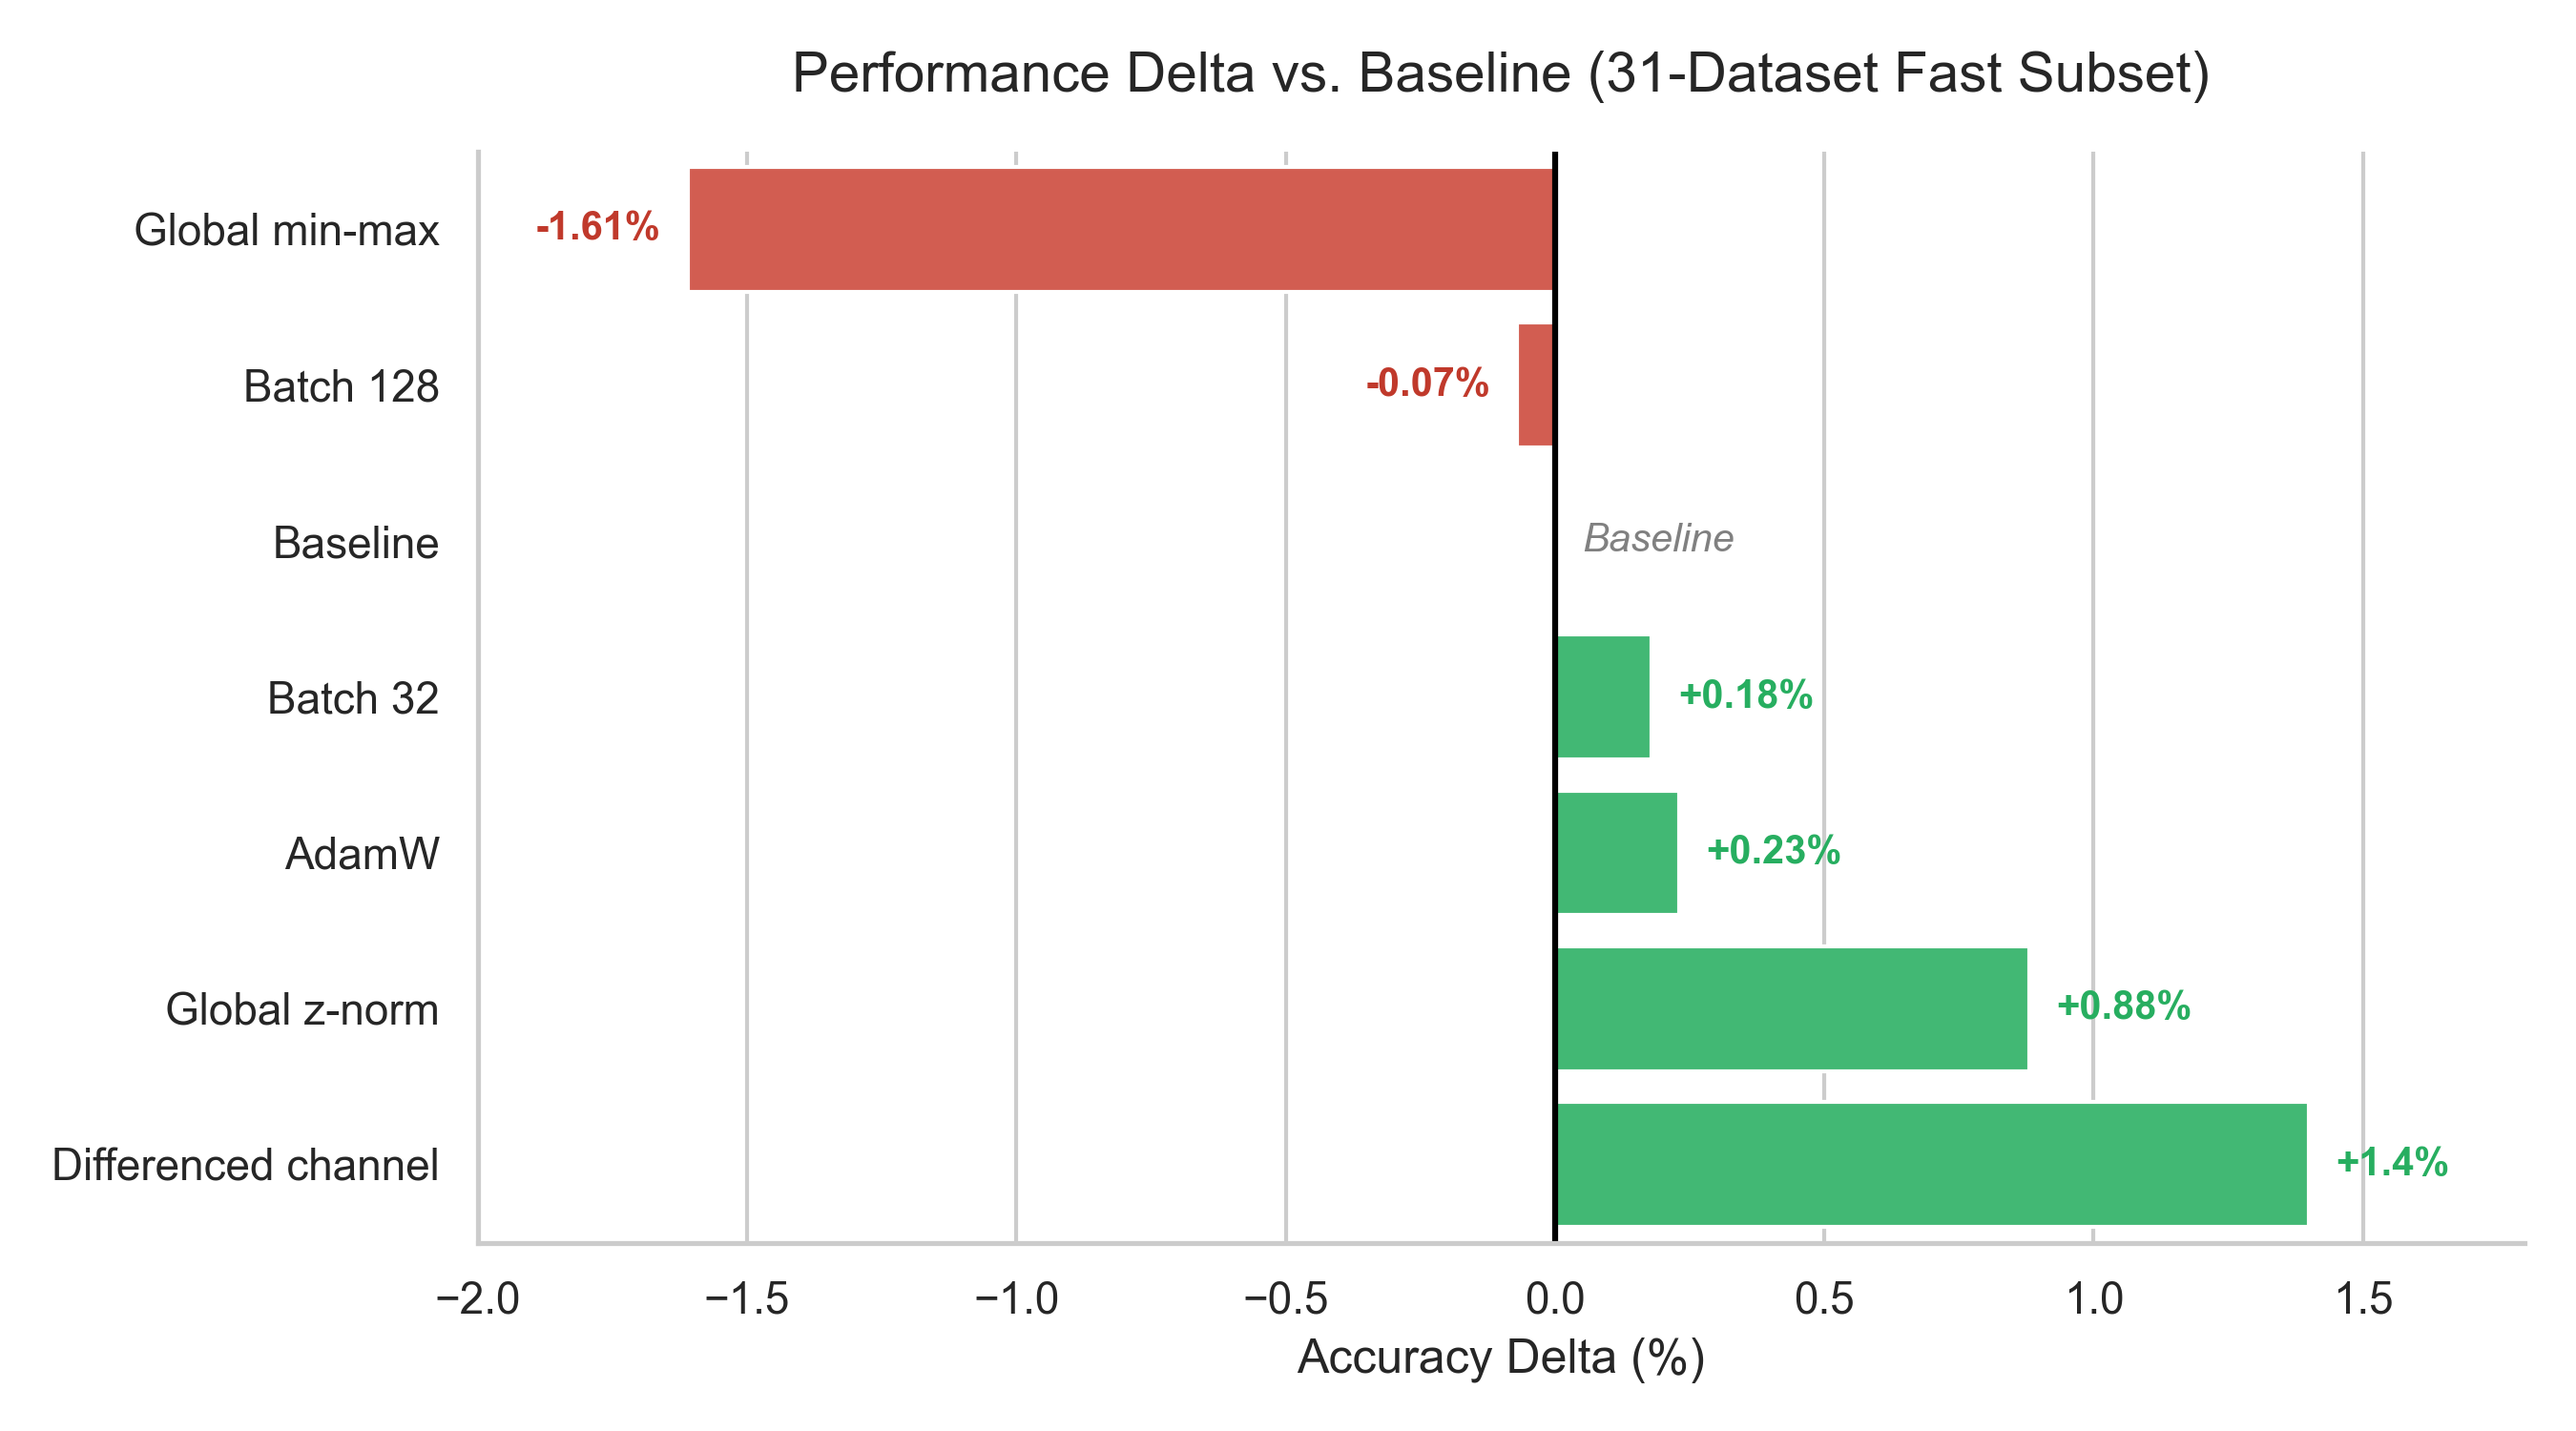
\includegraphics[width=\columnwidth]{../../plots/accuracy_comparison.png}}
    \caption{Mean accuracy comparison across improvement configurations.}
    \label{fig:accuracy_comparison}
\end{figure}

\begin{figure}[htbp]
    \centerline{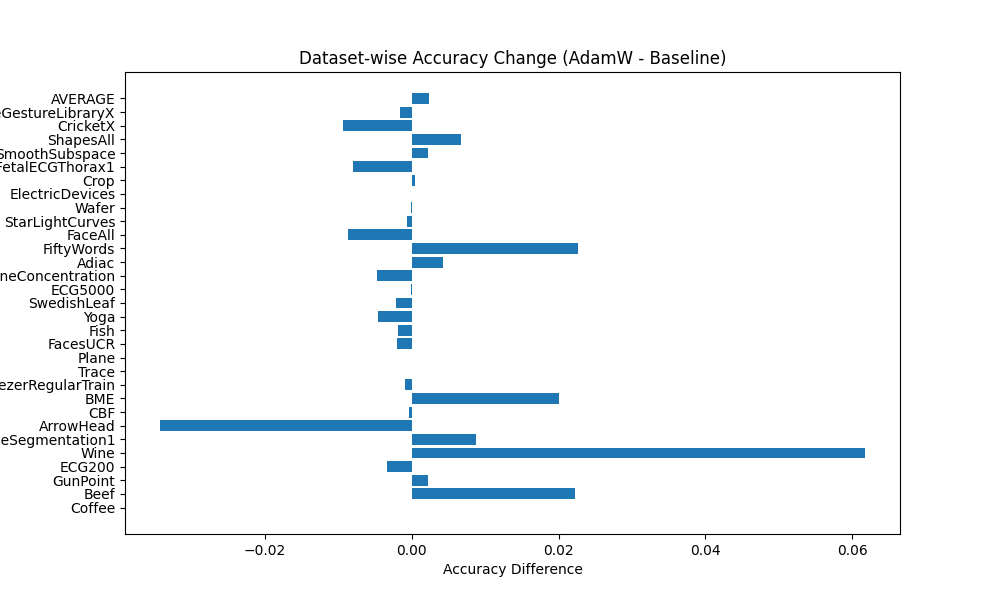
\includegraphics[width=\columnwidth]{../../plots/dataset_improvement.png}}
    \caption{Per-dataset accuracy improvement of AdamW over baseline.}
    \label{fig:dataset_improvement}
\end{figure}

\begin{figure}[htbp]
    \centerline{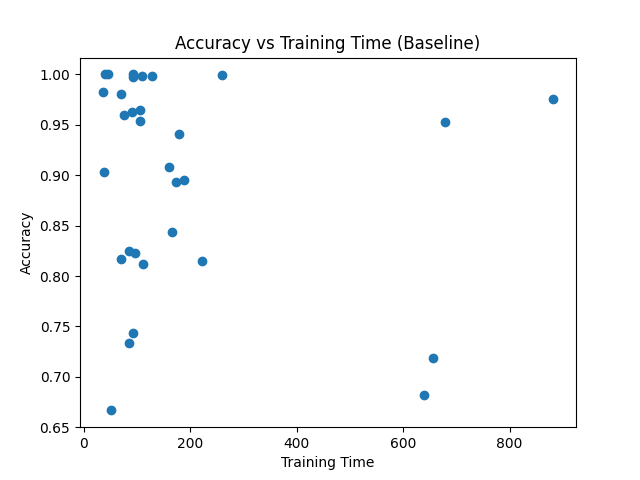
\includegraphics[width=\columnwidth]{../../plots/time_vs_accuracy.png}}
    \caption{Accuracy vs.\ training time trade-off across configurations.}
    \label{fig:time_vs_accuracy}
\end{figure}

\subsection{Ensemble Size Analysis}

Using the per-run predictions from the full 128-dataset evaluation, we analyzed how LITETime accuracy changes as the ensemble size $N$ grows from 1 to 10. Table~\ref{tab:ensemble} shows the results.

\begin{table}[htbp]
\caption{Effect of Ensemble Size on LITETime Mean Accuracy (128 UCR Datasets)}
\label{tab:ensemble}
\centering
\begin{tabular}{ccc}
\toprule
\textbf{Ensemble Size} & \textbf{Mean Accuracy} & \textbf{$\Delta$ from $N$=1} \\
\midrule
1 & 0.8317 & --- \\
2 & 0.8391 & +0.74\% \\
3 & 0.8422 & +1.05\% \\
4 & 0.8436 & +1.19\% \\
5 & 0.8445 & +1.28\% \\
6 & 0.8452 & +1.35\% \\
7 & 0.8456 & +1.39\% \\
8 & 0.8458 & +1.41\% \\
9 & \textbf{0.8461} & \textbf{+1.44\%} \\
10 & 0.8458 & +1.41\% \\
\bottomrule
\end{tabular}
\end{table}

The results reveal several important findings. Ensembling provides the largest marginal gain from $N$=1 to $N$=2 (+0.74\%), with rapidly diminishing returns thereafter. The accuracy plateaus around $N$=5--7, and slightly decreases at $N$=10, suggesting overfitting of the ensemble. The default choice of $N$=5 in LITETime is well-justified from a cost-performance perspective: it captures 89\% of the maximum ensemble benefit (1.28\% out of a maximum 1.44\%) while using half the compute of $N$=10.

\subsection{Multivariate Time Series Classification}

Table~\ref{tab:multivariate} extends the evaluation to 30 multivariate datasets. ConvTran achieves the highest mean accuracy (0.7383), followed by LITEMVTime (0.7100) and LITEMV (0.6965).

\begin{table}[htbp]
\caption{Mean Accuracy on 30 Multivariate Datasets}
\label{tab:multivariate}
\centering
\begin{tabular}{lc}
\toprule
\textbf{Method} & \textbf{Mean Accuracy} \\
\midrule
ConvTran & \textbf{0.7383} \\
LITEMVTime & 0.7100 \\
Disjoint-CNN & 0.7053 \\
LITEMV & 0.6965 \\
LITETime & 0.6937 \\
InceptionTime & 0.6895 \\
LITE & 0.6821 \\
FCN & 0.6770 \\
ResNet & 0.6720 \\
\bottomrule
\end{tabular}
\end{table}

LITEMV outperforms LITE on 16 out of 30 datasets (53\%), and LITEMVTime outperforms LITETime on 17 out of 30 (57\%), confirming that the multivariate-specific architecture provides a benefit for multi-channel inputs. However, ConvTran---which uses positional encoding with transformers---outperforms LITETime on 23 of 30 datasets (77\%), indicating that attention-based mechanisms capture cross-channel dependencies more effectively than the convolutional approach used in LITE/LITEMV.

Notably, LITE-family models still outperform FCN and ResNet, demonstrating their competitiveness even in the multivariate setting. The computational efficiency advantage of LITE models (significantly fewer parameters) remains relevant, particularly for applications where inference speed is critical.

%=============================================================================
\section{Discussion and Lessons Learned}
%=============================================================================

\textbf{Reproducibility verification.} The reproduction experiment confirmed the reliability of the original LITETime implementation. The mean accuracy difference of $<$0.15\% across 128 datasets demonstrates that the published results are robust to changes in hardware and software environment.

\textbf{Normalization matters more than optimizer choice.} The most impactful improvement was changing from per-sample to global z-normalization (+0.88\%), which outperformed optimizer changes (+0.23\% for AdamW). This finding is significant because normalization strategy is rarely the focus of ablation studies, yet it had the largest effect in our experiments. Global statistics provide more stable scaling, particularly for short time series where per-sample statistics may be unreliable.

\textbf{Environment and configuration challenges.} Reproducing deep learning results required careful attention to software versions, GPU configurations, and data loading pipelines. TensorFlow version differences and GPU-specific optimizations (mixed precision, XLA compilation) affected training behavior and required systematic configuration.

\textbf{Efficient experimentation.} The fast subset of 31 datasets enabled multiple configurations to be evaluated within limited computational budgets. This approach maintained evaluation diversity while reducing total runtime by approximately 75\%.

\textbf{Ensemble diminishing returns.} The ensemble analysis revealed that the default $N$=5 is near-optimal, capturing most of the ensemble benefit. Increasing beyond $N$=7 provides negligible improvement and can even slightly degrade performance, suggesting that redundancy in the ensemble predictions begins to dominate.

\textbf{Multivariate gap.} While LITE/LITEMV remain competitive with traditional deep learning methods (FCN, ResNet) on multivariate data, a significant gap exists with transformer-based architectures like ConvTran. This suggests that future lightweight architectures may benefit from incorporating attention mechanisms for cross-channel modeling.

%=============================================================================
\section{Limitations and Future Work}
%=============================================================================

Several limitations should be noted. The improvement experiments used a 31-dataset fast subset rather than the full 128-dataset archive. While carefully stratified, some configurations may behave differently on the complete benchmark. Additionally, this study focused on optimizer selection, batch-size tuning, and normalization strategies. Other hyperparameters---learning-rate scheduling (cosine annealing, cyclical LR), dropout rates, data augmentation, and architectural modifications (residual connections)---were not explored.

Hardware constraints limited the number of configurations tested. The computationally expensive nature of training across many datasets restricted the combinatorial exploration of hyperparameters.

Future work could extend this study in several directions:
\begin{itemize}
    \item Evaluating combined improvement strategies (e.g., AdamW + global z-normalization) to determine whether gains compound.
    \item Testing advanced learning-rate schedules such as cosine annealing with warm restarts.
    \item Exploring lightweight attention mechanisms to bridge the multivariate performance gap with transformer models.
    \item Applying automated hyperparameter optimization (Bayesian optimization) to identify optimal configurations efficiently.
    \item Evaluating on additional benchmark collections beyond UCR to assess generalization.
\end{itemize}

%=============================================================================
\section{Conclusion}
%=============================================================================

This project successfully reproduced the LITETime model and verified the reliability of its published results. The reproduced mean accuracy closely matched the reference value, demonstrating implementation stability under independent experimental conditions.

Improvement experiments revealed that normalization strategy has the largest impact on performance, with global z-normalization achieving the highest accuracy (+0.88\% over baseline). The AdamW optimizer provided a smaller but consistent improvement (+0.23\%) at no additional computational cost. Batch-size experiments confirmed the expected efficiency-accuracy trade-off.

The ensemble size analysis showed diminishing returns beyond 5 members, validating the default LITETime configuration. The multivariate extension demonstrated that LITE-family models remain competitive with traditional deep learning methods but lag behind transformer-based architectures on cross-channel modeling.

Overall, these findings confirm that lightweight architectures remain strong candidates for time series classification, particularly in resource-constrained environments. Meaningful performance improvements can be achieved through careful optimization without modifying the core architecture, highlighting the importance of preprocessing and training configuration in deep learning research.

%=============================================================================
\section*{Work Plan and Contribution}
%=============================================================================

This project was completed collaboratively over an eight-week period. Table~\ref{tab:workplan} summarizes the project timeline.

\begin{table}[htbp]
\caption{Project Timeline and Responsibilities}
\label{tab:workplan}
\centering
\small
\begin{tabular}{lll}
\toprule
\textbf{Phase} & \textbf{Duration} & \textbf{Lead} \\
\midrule
Paper Selection & Week 1 & All Members \\
Environment Setup & Week 2 & All Members \\
Dataset Preparation & Week 2 & All Members \\
Baseline Reproduction & Weeks 3--4 & All Members \\
Fast Subset Creation & Week 4 & All Members \\
Optimizer Experiments & Week 5 & All Members \\
Batch Size Experiments & Week 5 & All Members \\
Normalization Experiments & Week 6 & All Members \\
Multivariate Evaluation & Week 6 & All Members \\
Visualization \& Analysis & Week 7 & All Members \\
Report Writing & Weeks 7--8 & All Members \\
Final Review \& Submission & Week 8 & All Members \\
\bottomrule
\end{tabular}
\end{table}

\textbf{Contribution Summary.}

\textbf{Kiran Meenakshi Sundaram} contributed to dataset preparation, implementation integration, experiment execution, GitHub repository development, and report preparation.

\textbf{Jos\'e Ram\'on Morera Campos} contributed to baseline reproduction, improvement experiments, optimizer tuning, normalization and batch-size evaluation, and code development.

\textbf{Pelayo Garc\'ia \'Alvarez} contributed to result analysis, visualization, interpretation of experimental outcomes, multivariate evaluation, and refinement of written sections.

All members participated in reviewing the experimental methodology, validating results, and finalizing the submission.

%=============================================================================
\begin{thebibliography}{00}

\bibitem{ismail2024lite} A.~Ismail-Fawaz, M.~Devanne, S.~Berretti, J.~Weber, and G.~Forestier, ``Look into the LITE in deep learning for time series classification,'' \textit{International Journal of Data Science and Analytics}, pp.~1--21, 2025.

\bibitem{dau2019ucr} H.~Dau et al., ``The UCR Time Series Classification Archive,'' 2018. [Online]. Available: \url{https://www.cs.ucr.edu/~eamonn/time_series_data_2018/}

\bibitem{wang2017fcn} Z.~Wang, W.~Yan, and T.~Oates, ``Time series classification from scratch with deep neural networks: A strong baseline,'' in \textit{International Joint Conference on Neural Networks (IJCNN)}, 2017.

\bibitem{fawaz2019deep} H.~Ismail Fawaz et al., ``Deep learning for time series classification: A review,'' \textit{Data Mining and Knowledge Discovery}, vol.~33, pp.~917--963, 2019.

\bibitem{fawaz2020inceptiontime} H.~Ismail Fawaz et al., ``InceptionTime: Finding AlexNet for time series classification,'' \textit{Data Mining and Knowledge Discovery}, vol.~34, pp.~1936--1962, 2020.

\bibitem{loshchilov2019adamw} I.~Loshchilov and F.~Hutter, ``Decoupled weight decay regularization,'' in \textit{International Conference on Learning Representations (ICLR)}, 2019.

\bibitem{keogh2001dtw} E.~Keogh and M.~Pazzani, ``Derivative dynamic time warping,'' in \textit{SIAM International Conference on Data Mining}, 2001.

\bibitem{dempster2020rocket} A.~Dempster, F.~Petitjean, and G.~Webb, ``ROCKET: Exceptionally fast and accurate time series classification using random convolutional kernels,'' \textit{Data Mining and Knowledge Discovery}, vol.~34, pp.~1454--1495, 2020.

\bibitem{dempster2021minirocket} A.~Dempster, D.~Schmidt, and G.~Webb, ``MiniRocket: A very fast (almost) deterministic transform for time series classification,'' in \textit{ACM SIGKDD}, 2021.

\bibitem{tan2022multirocket} C.~W.~Tan, A.~Dempster, C.~Bergmeir, and G.~Webb, ``MultiRocket: Multiple pooling operators and transformations for fast and effective time series classification,'' \textit{Data Mining and Knowledge Discovery}, 2022.

\bibitem{aeon2024} Aeon Toolkit, ``Aeon: A Python toolkit for learning from time series,'' 2024. [Online]. Available: \url{https://www.aeon-toolkit.org/}

\bibitem{bagnall2017bakeoff} A.~Bagnall et al., ``The great time series classification bake off: A review and experimental evaluation of recent algorithmic advances,'' \textit{Data Mining and Knowledge Discovery}, 2017.

\bibitem{lines2012shapelet} J.~Lines et al., ``A shapelet transform for time series classification,'' in \textit{ACM SIGKDD}, 2012.

\bibitem{foumani2023convtran} N.~Mohammadi Foumani et al., ``Improving position encoding of transformers for multivariate time series classification,'' \textit{Data Mining and Knowledge Discovery}, 2023.

\bibitem{zhao2017cnn_tsc} S.~Zhao et al., ``Convolutional neural networks for time series classification,'' \textit{IEEE Transactions on Industrial Informatics}, 2017.

\bibitem{pineau2021reproducibility} J.~Pineau et al., ``Improving reproducibility in machine learning research,'' \textit{JMLR}, vol.~22, pp.~1--20, 2021.

\end{thebibliography}

\end{document}
